\chapter{Regionally Containing Epidemics: Modelling Ash dieback}

% paper title: Large-scale control based on regional containment
% there is a surprising lack of, simplified, ash dieback models in the literature...\ciations... <-- double, triple and quadruple check!
% without host demography 
% landscape level control strategy

Previously in Chapter \ref{ch5:dispersal-model}, we considered a generic $SIR$ model that spread via wind-borne dispersal. Constructing the dispersal model resolved the major problem witnessed in Chapter \ref{fig:ch4_uk_spread}, namely, the failure of the SLM to spread on a realistic host density. However, the findings of Chapter \ref{ch5:dispersal-model} lacked biological specificity and thus, came short of aiding plant health. In this chapter, I will aim to address this. The present chapter will construct a simplified model of ash dieback, based on the dispersal model, and be utilised to develop an epidemic control strategy.

There has been a great deal of work carried out into the nature of control in plant and tree-based epidemics\footnote{See section \ref{chapter2:plant-ecologoy} for a review on the control in plant-based epidemics.}. In particular, the spatial structure of plant-hosts is an essential factor when considering how to manage an outbreak \cite{spatial-control-optimisation, control-heterogeneous-landscapes}. The accepted paradigm of control typically considers infected tree removals over a relatively small spatial scale, near infected hosts \cite{WEBIDEMICS}, or more broadly, ahead of the wavefront \cite{large-scale-control}. However, landscape-level epidemic control, based solely on the structure of large-scale spatial distribution of hosts incorporating topography, has yet to be explored in-depth.\\

As such, in this chapter, we will examine how host-heterogeneity, under the influence of a wind-dispersed pathogen, can give rise to natural pinch-points and fault lines in the spatial distribution of hosts. Population pinch points may give rise to a bottleneck in the epidemic spread, which in principle, may be exploited with targeted tree felling to fragment the host population with minimised effort. In essence, a strategy of 'regional containment', targeting the local wind-based pathogen dispersal mechanism, is formulated and scaled up over large spatial scales. Similar concepts for crop and livestock diseases have been outlined \cite{PAPAIX201435, GILIOLI20131, Gilligan-disease-management}, however, to our knowledge, this has not been generalised to tree population distributions over large spatial scales.

A simplified $SEIR$-type model of ash dieback is developed to demonstrate this control strategy, alongside an appropriate definition of the reproductive ratio\textemdash denoted by $R_0$. The value of $R_0$ is projected onto the map of ash tree canopy cover in GB, as given by \cite{hill.data}. From the $R_0$ maps we construct, a simple notion of epidemiological connectivity can be defined and visualised through a susceptible '$R_0$-cluster' over the population of GB ash trees. This leads us to develop a heuristically-based fragmentation algorithm. As we define it, fragmentation considers which locations in the population, if artificially taken below $R_0 = 1$ through felling, would disrupt epidemiological connectivity\textemdash, thus leading to containment. Epidemic containment in the largest $R_0$-cluster is then analysed and shown to be most applicable over a specific range of infectivity parameters.


% multi-scale approaches have been outlined \cite{hart2020theoretical}
% multi-seasonal frameworks comprise a common theme in the spread of crop-based epidemics see  x, y, and typically involve soil-borne nematodes-based outbreaks \cite{tankam2020modelling} <- see references inside.
% ash dieback has a strong morality rate \cite{stocks2017first}

\section{Methods}

\subsection{On the biology of ash dieback}

Ash dieback, caused by the fungus \textit{H.pseudoalbidus} (HP), is a highly seasonal \cite{bengtsson2014seasonal} and follows a complicated, yearly, polycyclic infection cycle. The ADB pathosystem, commonly referred to as \textit{H.pseudoalbidus}-\textit{F. excelsior}, has been the subject of much research over the years, the taxonomy, symptoms and life-cycle of the pathogen are well-known \cite{https://doi.org/10.1111/mpp.12073}. However, there is a noticeable absence of ADB modelling in the literature. 

A tree infected by HP will shed its leaves in the Autumn; fruiting bodies will then proceed to grow on the leaf debris from the tree's previous years growth cycle and sporulate in the summer, thus leading to new secondary infections. Although a complete description of the pathosystem is beyond the scope of this chapter, the life-cycle can be understood to have two phases of growth, sexual and asexual. The asexual phase occurs when the pathogen infects and amplifies through the host \textcolor{red}{and occurs all year round}. The sexual phase of HP occurs during the summer months, from June until September when wind-dispersed spores infect new ash trees. 

\subsection{Constructing an $SEIR$ model}


\begin{table}[h]
\centering
\begin{tabular}{l l l}
\hline
\textbf{Model parameter} & \textbf{Description} & \textbf{Typical value(s)}\\
\hline
$\rho$  & Tree density & $0.00 - 0.10$ \\ 
$\beta$ & Infectivity & $0.00010 - 0.00100\ \mathrm{day}^{-1}$ \\
$\phi$ & Sporulation peak & Occurs in $[\mathrm{June}, \mathrm{September}]$  \\
$\ell_{ga}$ & Pathogen dispersal distance & $196\mathrm{m}$ \\
$T$ & Sporulation peak & $120$ days from June - September \\
$t$ & Time-step & $[0, T]$ days\\
$R_0$ & Mean reproduction number & $0-20$ \\
$\mathcal{L}$ & Lattice dimension & $1000\times1000$ \\
$\mathcal{A}$ & Domain area & $5\mathrm{km}\times5\mathrm{km}$ \\
$\gamma$ & Lattice constant & $5\mathrm{m}$ \\
$\mu$ & Peak leaf-shedding of ash & November \\
$\sigma$ & Leaf-shedding standard deviations & 2 weeks \\

\hline
\end{tabular}
\caption{Model parameters}
\end{table}

\begin{figure}
    \centering
    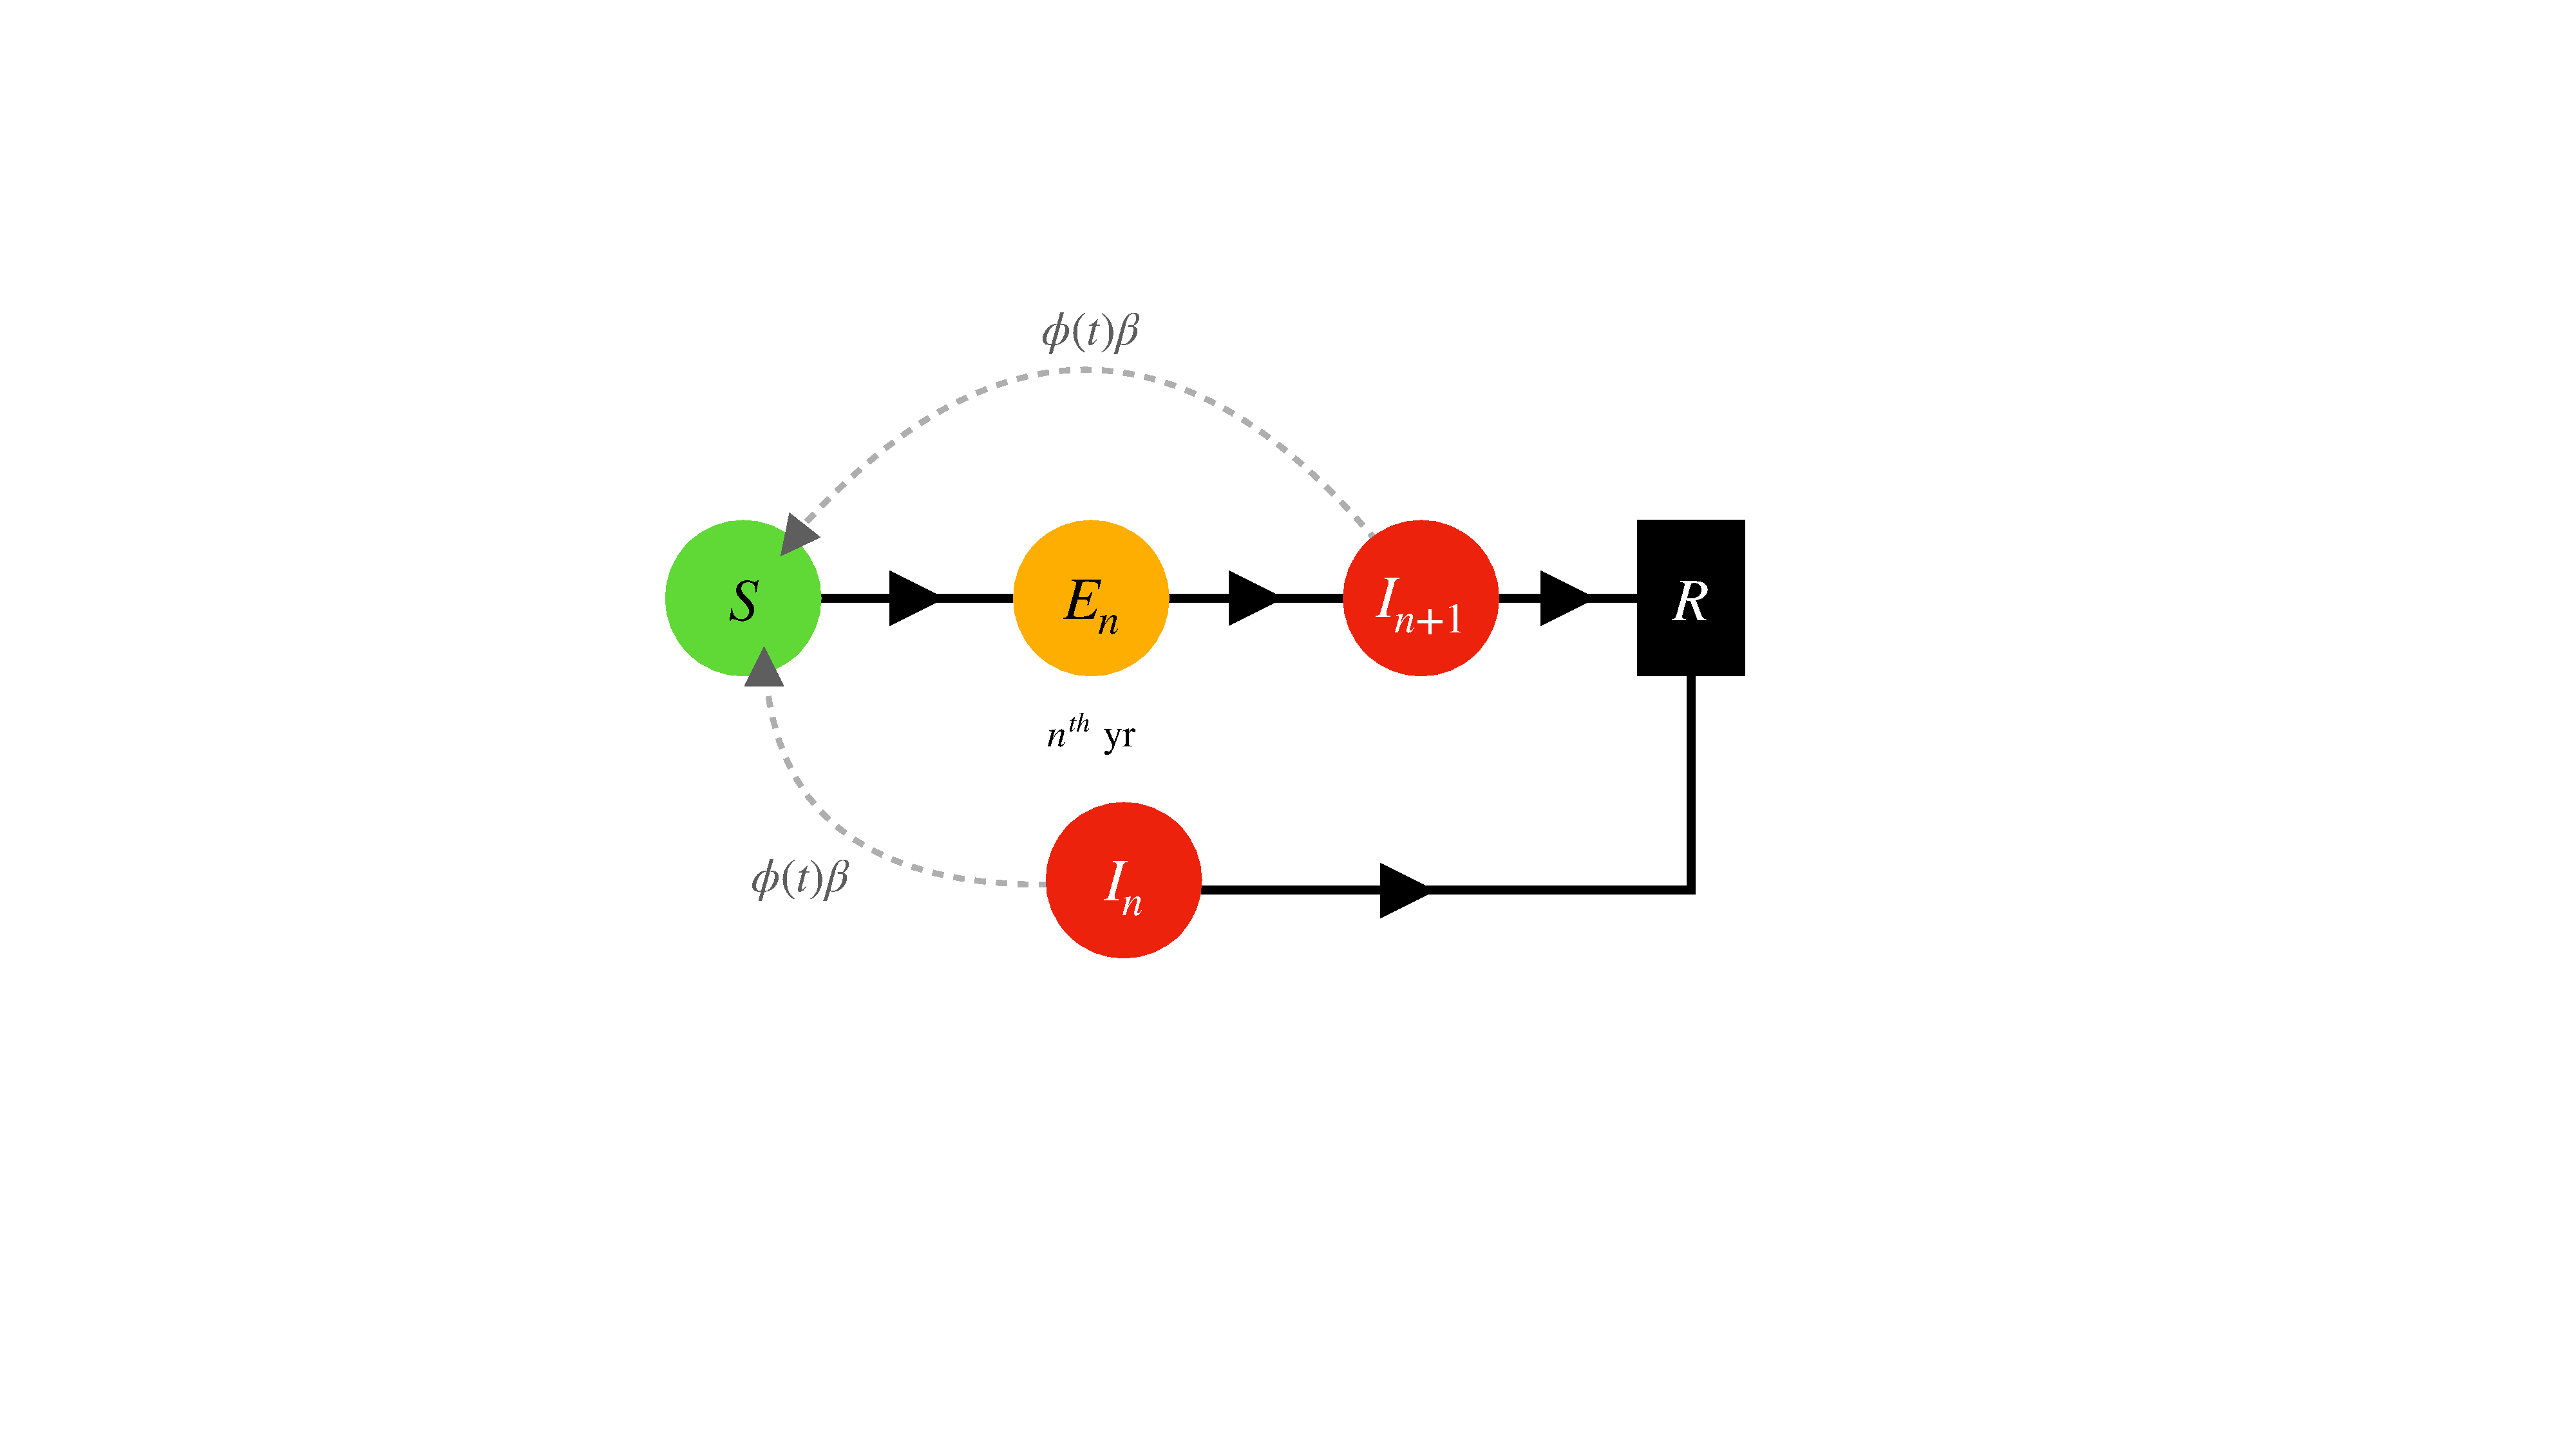
\includegraphics[scale=0.30]{chapter6/figures/fig1.pdf}
    \caption{The $SEIR$ model of ash dieback. In the $n^{th}$ year of an outbreak, an infectious tree may cause a transition $S\rightarrow E_n$, depicted by the bottom dashed grey arrow. A tree that becomes latently infected in year $n$ will lead to an infectious tree in year $n+1$. Eventually, all infected ash are removed without the possibility of recovery.}
    \label{fig:my_label}
\end{figure}

As before, the hosts distribution, in this case, ash trees, is seeded by a Bernoulli trial with probability $\rho$ according to a binomial distribution\textemdash, thus giving rise to a flat, randomly distributed landscape of trees. The probability $\rho$ defines the host density inside a square domain of size $\mathcal{L}$. Each lattice point is chosen to represent a $5\mathrm{m}\times5\mathrm{m}$ patch of land that approximates the canopy cover of an ash tree \cite{ash-tree2, ash-tree1}, this resolution yields an upper bound of $400$ ash trees per hectare of canopy cover.

However, this time, we include an extra latently infected (or exposed) compartment, denoted by $\ell$, into the model. Thus, a tree can be in one of four compartments and trees transition through $S\rightarrow E \rightarrow I \rightarrow R$, without the possibility of recovery. The inclusion of an exposed category is included to reflect the biological life-cycle of HF and the period of time of time whereby an infected ash tree may display symptoms, but crucially remains noninfectious. The probably of transition from $E\rightarrow I$ is set by a Gaussian distribution, centered on November with variance 2-weeks \textcolor{red}{citations}. This choice of parameters represents the seasonal shedding of leaves in Autumn, at which point, the latently infected ash tree taken to become infectious. 

The life cycle of 
We consider two dispersal kernels, a thin-tailed Gaussian and a fat-tailed power-lower.

Given two trees, one susceptible ($S_x$) and one infected ($I_{x^\prime}$), separated by a distance $r$, an expected transition rate for $S_x \rightarrow E_x$ can be determined from the dispersal kernel multiplied by an infectivity rate $\beta$. For Gaussian and power-law this assumes the form:

\begin{equation}
    Pr(S_{x} \rightarrow E_{x} ;\ I_{x^{\prime}} ) = \beta  \phi(T) \exp\Big[\frac{-r^2}{2\ell^2}\Big] 
\end{equation}
\begin{equation}
    Pr(S_{x} \rightarrow E_{x} ;\ I_{x^{\prime}} ) = \beta \phi(T) (1 - r/\ell)^{-r}
\end{equation}

% beta is a per-capita rate of infection, that can be seen as a compound parameter...

A simple time-dependant function $\phi(T)$ takes the value of $1$ between the summer months of June - September, and $0$ otherwise thus reflecting the sporulation peak of \textit{Hymenoscyphus fraxineus} (HF). During these summer months, wind-borne dispersal occurs when fruiting bodies produce large numbers of ascospores. 

We make an assumption that trees transitioning from $E\rightarrow E; I_{n}$
We make an assumption that trees transitioning from $S\rightarrow E$ on account of infected tree $I_{n}$, will only become infectious to neighbouring trees during the following sporulation peak, denoted by $S\rightarrow E; I_{n+1}$. This is justified given the strong seasonal component in the life cycle of \textit{Hymenoscyphus fraxineus}\textemdash that is, where infected trees shed plant-material which 
becomes infectious during the following sporulation peak. 

% Typically an infected ash tree may expect to survive for around x years before death, this time-scale is beyond what we consider here - why ?

% Ash dieback is known to sporulate in the summer months... therefore...

% subdividing compartments in this manor could also provide an easier implementation to hosts which become more infectious, through a greater production of spores, as the infectious cycle continues not to mention particular periods of environmental unsuitability.
% Individuals in different compartments, (e.g. E_2 vs E_3 and so on) are not biologically different, they are merely in different states of infection. 

%  Thus, we assume an infected tree is the dispersal site. In contrast, a real-life scenario may first involve the dispersal of infected leaves following the dispersal of fungi spores. We discuss the consequences of this assumption later. % exists in that shed/dead plant material remain fixed at the hosts spatial location. 
 
\subsection{Defining $R_0$}

% R0 is the measure used to capture the pathogens ability to invade
% Q: what is the relationship between the mortality ratio (or final fraction of infected hosts) ? 
% If R0 was considered over a larger time-scale, host-regrowth would need to be integrated into the model
% Furthermore, measuring R0 over a larger time-scale could over, or underestimate, the degree to which a response would need to be undertaken in the response time-window. 
% a basic reproduction number $R_0$ is defined for the first life-cycle of the pathogen.
% Moreover, data over a relatively short time scale is typically all that is available when making decisions about control, not to mention the added complexity of incorporating host-regrowth–which becomes an important factor over longer time scales–and so, the constraint of computing R0 over longer time scales is relaxed. 
%  We develop the simplest implementation possible, namely, where R_0 is measured over one pathogen life-cycle, and the course of infection for each host follows the same process with perfect fidelity. This lies in stark contrast to a realistic scenario whereby different hosts show considerable differences.


\begin{itemize}
    \item see for a review on how R0 is calculated \cite{perspectives-on-r0}, we use method x in order to estimate and inform R0
    \item $R_0$ is a complex function which changes in time, to this end, the next generation operator is used to derive a value for $R_0$ \cite{doi:10.1098/rsif.2009.0386}. In order to inform the value of $R_0$ we do xy and z...
    \item Although it is hard to enforce a true $R_0$ value, the most important feature introduced from the definition is a threshold from which we can see if a local invasion is likely to take place.
    \item Since the number of susceptible hosts is fixed, without replacement, the number of susceptible hosts will continually decrease in time in the case of an epidemic. Given the strong spatial component in the model we expect that measuring $R_0$ as-per this definition will give an under-estimate for later times when few susceptible trees remain. Likewise, for earlier times when susceptible neighbours are plentiful $R_0$ will yield an upper estimate for the pathogen. In order to characterise the pathogen in this model, we take the upper bound defined between the $1^{st}-2^{nd}$ generations. This simplification represents a worst-case scenario and the mean value of $R_0$ would be lower for later times when there are less trees available to infect. But most importantly, the threshold of transmission $R_0>1$ is reliable captured \textit{during the initial stage of infection}.
    \item $R_0$ can be fully characterised by a growth rate \cite{R0-construct}. That is, the growth factor per generation.
    
\end{itemize}

In this Chapter aspects of the sub-grid model are improved.
\section{The biology of Ash dieback} % why not remain with Oak?
\begin{itemize}
    \item review: \cite{ash-dieback-costs}
    \item review: \cite{doi:10.1111/1365-2745.13383}
    \item review: \cite{ash-tree1}
\end{itemize}

\subsection{Constructing $R_0$-maps}

\begin{figure}
    \centering
    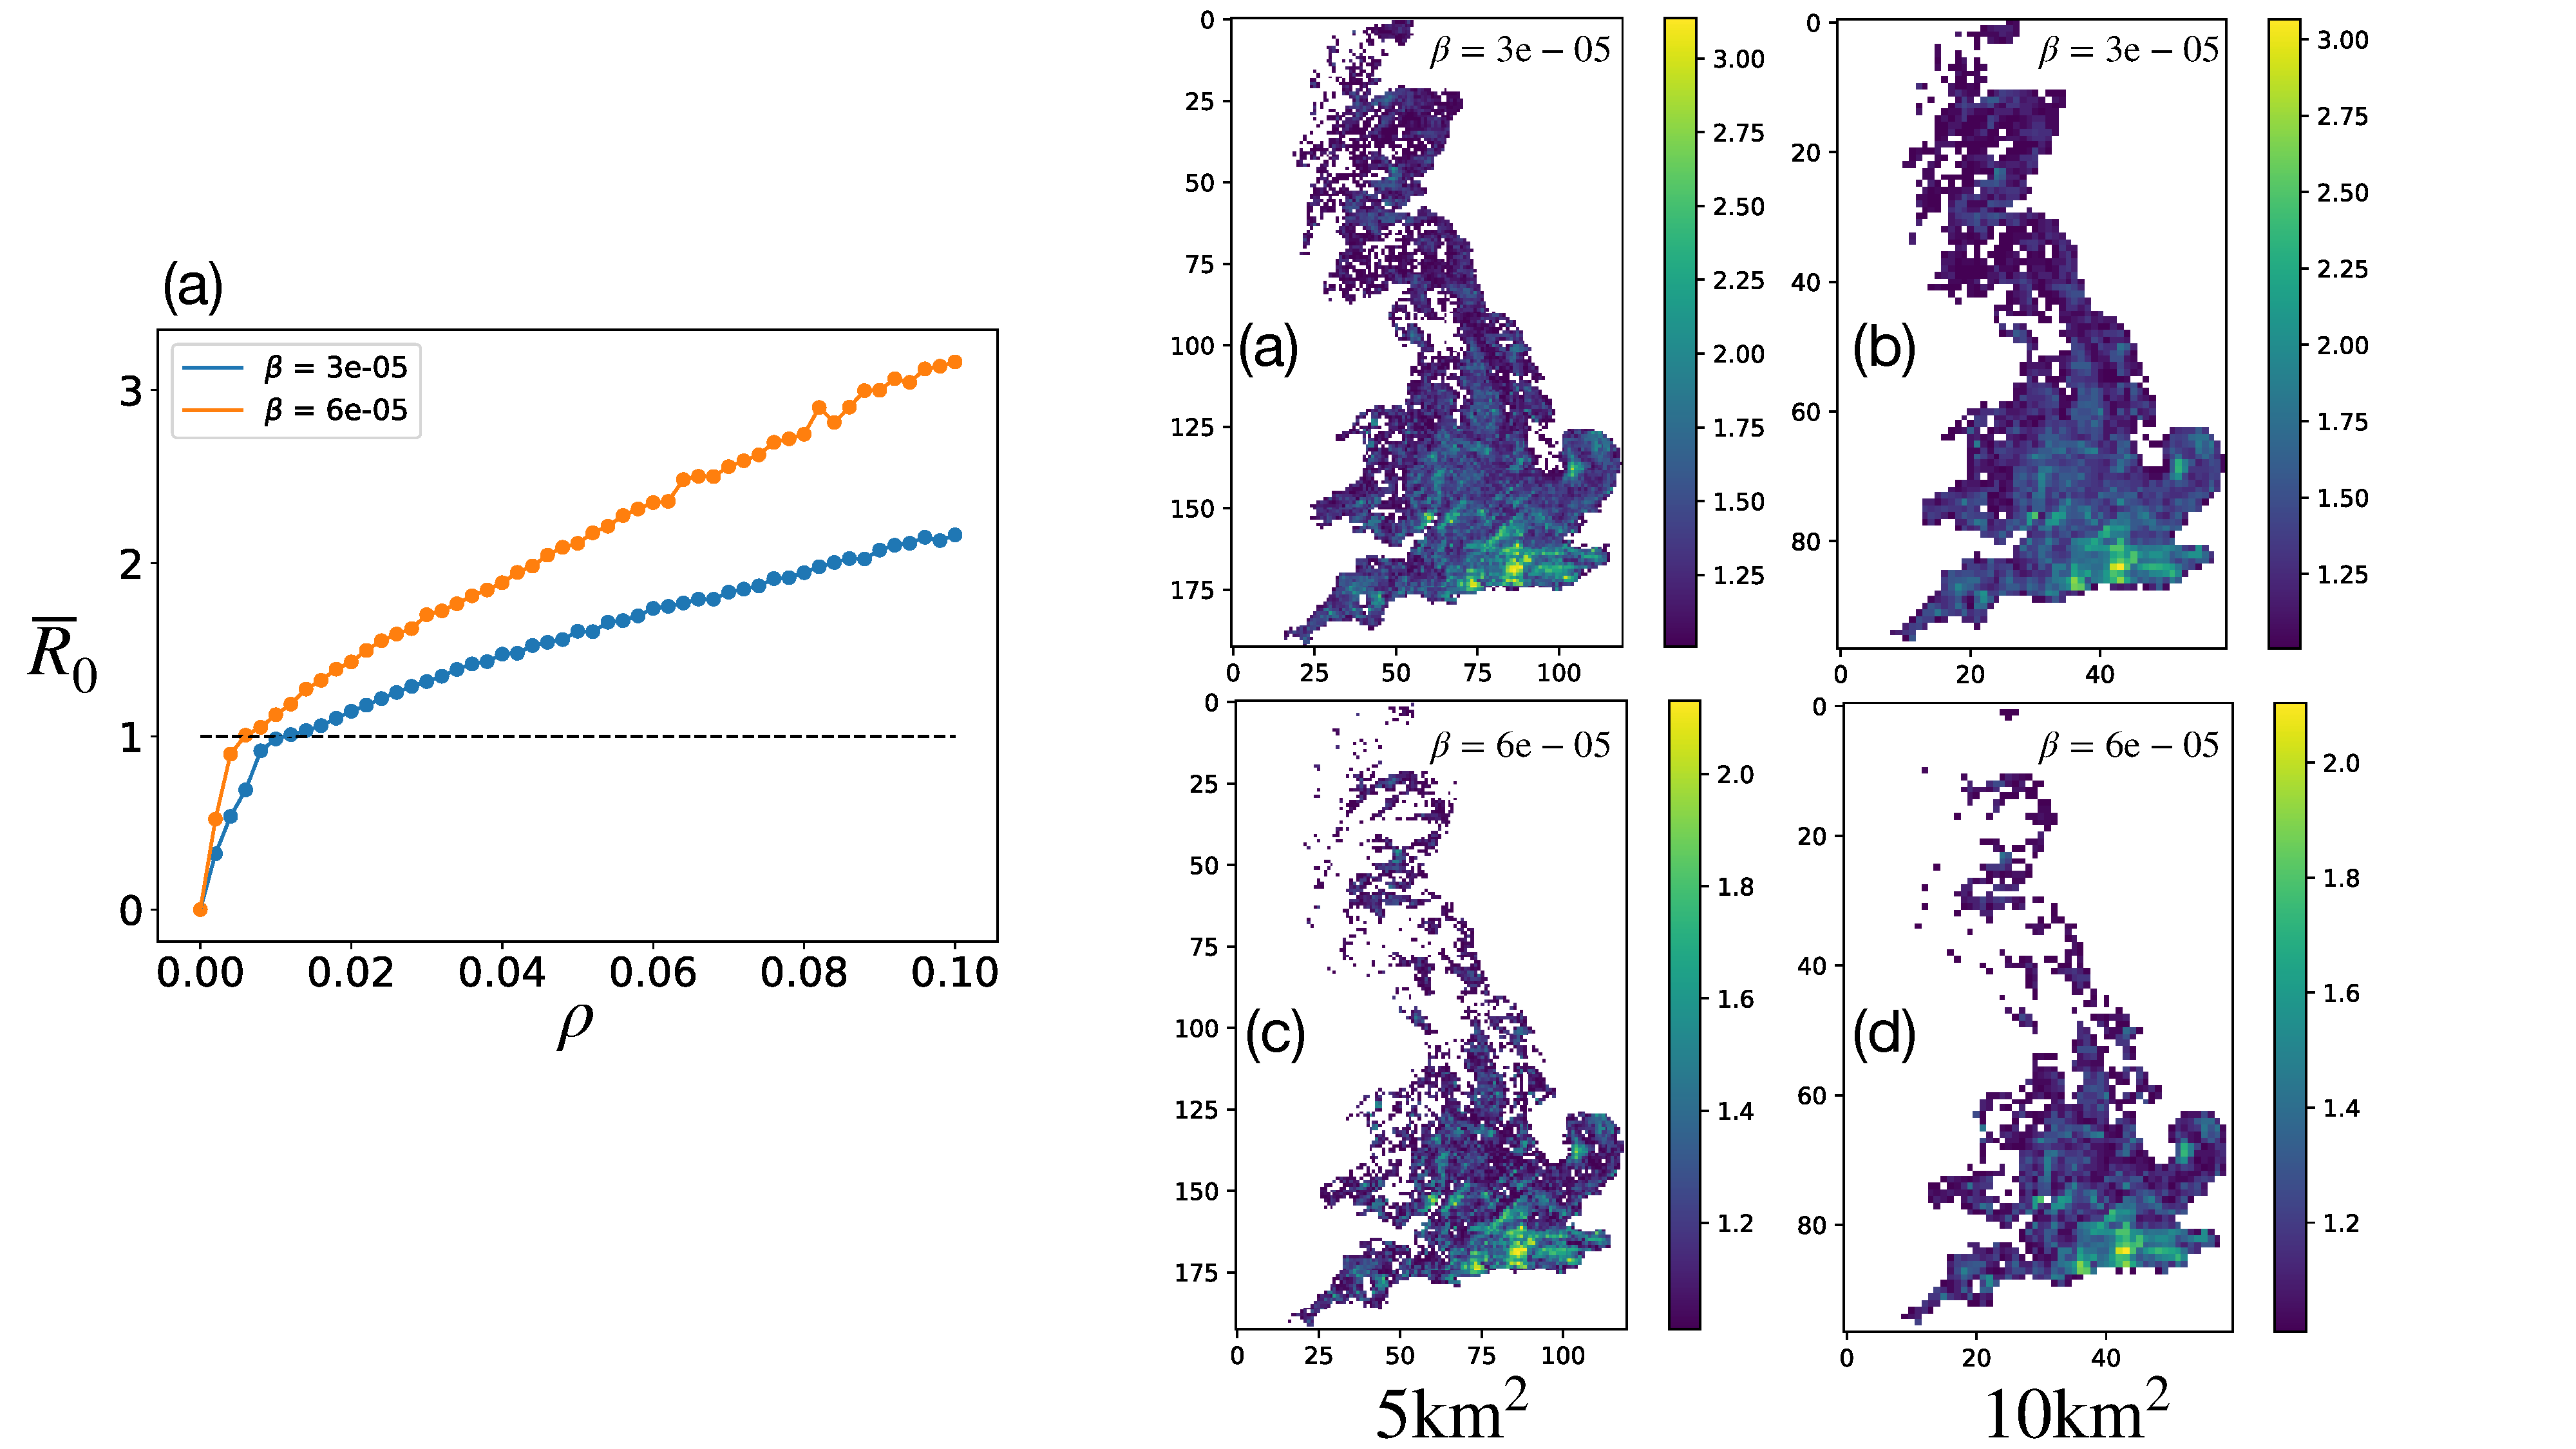
\includegraphics[scale=0.25]{chapter6/figures/fig2.pdf}
      \caption{(a) Ensemble-averaged $R_0$ between two values of $\beta$, for Gaussian dispersal of $\ell=1.6\mathrm{km}$. (a-b) $R_0$-map for $\beta=3\mathrm{e}-05$, coarse-grained at $5$, $ 10\mathrm{km^2}$. (c-d) $R_0$-map for $\beta=6\mathrm{e}-05$.}
    \label{fig:my_label}
\end{figure}

\section{Chapter summary}

\textbf{Model improvements...}
\begin{itemize}
    \item 
    \item introduce the regime of pathogen spread we are interested in, we are not modelling continental long-range spread via upper atmosphere, nor are we interested in long-range human trade networks. We are interested in dispersal at the local level whereby passive means of wind, soil and or insects/animals. 
\end{itemize}


% Where we consider spatial structure and others have not
% - In this chapter, we focused on disrupting local-level dispersal by implementing control at landscape-level.
% -  In this chapter we undertook the ambitious task of scaling up a small-scale model, to large spatial distances covering GB, and developed a new approach to controlling the spread of disease.

These results are focused toward help policy makers implement informed decisions, about \textit{where} to control the spread of disease, based on spatial arguments, when budgets are low\textemdash as noted by \cite{time-varying-infectivity}. Our approach of spatially scaling small-scale epidemiological principles was conducted through computational, opposed to analytical, means. 

The article published by \cite{time-varying-infectivity} indicates the possibility of \textit{preferentially} controlling an area based on the final-sized epidemic. It goes without saying that areas of land that have the largest final sized epidemic are likely the most density populated. However, we outline the possibility it might be more beneficial to preferentially control an area based on its spatial location and how it couples to to neighbouring areas.

% The scaling up of our model
The scaling up of our model resembles a metapopulation model, now commonplace when modelling plant-based epidemics, but crucially our large-scale model is not dynamic. A dynamic large-scale model is indeed useful for the prediction of time-scales and the movement of disease-fronts movement; however, we suggest they might be at best less useful for optimised large-scale control, and at worse, nicely complemented by the approach we develop.

If early data through a particular region, with known data, was collected, it would be a relatively short step to fit the dispersal model and scale up the model over large distances given the seemingly simple relation to host density $\rho$.
% At the small scale we have a uniform population. However for larger scales we have considerable spatial heterogeneity.
% spatial-scale and control, over a multi-seasonal pathosystem, have been investigated for sugar beet in the UK, see \cite{doi:10.1146/annurev.phyto.45.062806.094357} for a review.

% On the SEIR model

The cyclic nature of the $SEIR$-type model constructed in this article can also find resemblance in the, well established body of literature, of crop-based epidemics. It is common-place for a field of crops to become infested, then at the end of the growing season be totally eradicated by virtue of harvesting % \cite{time-varying-infectivity} has 
% we contend the SnIEmR model, considered over one sporulation peak, is a simplistic implementation of the SEIR-based model needed to compute an invasion threshold that represent the infection dynamics ash dieback. 
% The SEIR-based model is made more flexible, and can be readily extended or adapted to incorporate more biological realism, by virtue of splitting the E and I into multiple compartments\textemdash this is frequently done in human and animal-based models \citations..

%- Although the main result of our work was conduced over one sporulation peak, or life-cycle of ash dieback, splitting the model into various compartments was a useful and necessary step towards developing accurate large-tree species. reference  \cite{https://doi.org/10.1111/ppa.12894} alludes to multiple exposed periods being useful

%- A quantity of interest that appears frequently in the literature is the initial growth rate $r$, that is the density-independent growth at the start of any epidemic.
% See \cite{ferrandino2012time} for a review on the time-scales and sporulation of plant-based diseases.

% Fitting data to the early phases of an epidemic has been shown to give large differences in the final-size epidemic, or severity \cite{time-varying-infectivity}. However, we are only interested in a pathogens ability to invade and this can be closely approximated by measuring R0 over the fist observation (\see appendix)

% The variability between the particular life-cycle history followed by hosts is thought to be an important factor to consider\cite{ferrandino2012time}, and we intentionally neglected this for the purpose of simplicity...

% Main assumptions in the method: 
% 1) Assumptions about dispersal
Dispersal over small spatial-scale is thought to predominately occur passively through wind, however other means of dispersal exist such as soil and or insects. There are many pathways a pathogen can use to spread through a landscape, including long-range dispersal, mediated through either human-trade networks %
\cite{hulme2009trade, banks2015role, chapman2017global} or dispersal in the upper atmosphere \cite{westbrook1999atmospheric, isard2005principles}.  

% We assumed some regions can sustain an epidemic and some cannot, we assume that $R_0>1$ is the threshold separating these regimes.

% 2) Assumptions about R0
To our knowledge, $R_0$ has not been estimated for Ash dieback, or indeed for any large deciduous tree species, unlike for some crop-based pathogens \cite{segarra2001epidemic}. The lack of $R_0$-estimates made it hard to scrutinize which $\beta$-valued $R_0$-map would be likely to reflect reality. This gap in the body of literature is hardly surprising given the complexity of measuring time-varying infectivity rates \cite{13-challenges}. Thus, as it stands, our results hint-towards the utility of landscape-level control but come short of definitive proof.

% Looking at \cite{R0-perc-ref}, it makes me think our notion of $R_0$ is pretty simplistic. We only measure the local-level $R_0$. We do not consider $R_0$ from patch to patch. What scale we measure $R_0$ has a huge impact on what the result is. Could we rank land-patches not only on there local $R_0$ level, but also on the impact they have on there immediate neighbours ? This would, in theory be an improvement to the clustering algorithm.

% Improvements to the model:
% 1) The algorithm
% The algorithm to target not only the critically connecting patches, but also find fragmenting lines which minimise risk at the landscape-level ? Incorporating the local impact a particular patch may have on its neighbours.
% 2) Multi-year R0 analysis
% However, we .... xyz cover all basis of using a one-season approximation. <- this leads to a risk-based argument in which we could capture a 2nd-order R0 which does, xyz. We mainly interested in a pathogens ability to invade. 

% Analysis was aired towards simplicity, a more expansive study with e.g. more sophisticated sporulation functions could be the subject of future work.

% The most important message of our work was...
% The spatial and temporal scale of the control-strategy should match intrinsic spatial and temporal scale of the invasion. <- Hence R0 measured over one season. 


% our modelling approach and results are in their infancy,  

% Last remarks and future modelling work:
To our knowledge, there is a surprising lack of spatio-temporal ADB models exist in the literature, probably because of the significant challenges involved in containment. Although our findings are far from complete, it suggests the spread of ash dieback, between spatial locations, could be reduced by preferentially targeting sites to minimise epidemiological connectivity. Not surprisingly, more work will need to be done to ascertain the degree to which this strategy could impede the spread. 

% Crucially, future work will involve integrating LDD mechanisms into the model in order to understand the relative importance long vs local distance dispersal. We may speculate about the relative importance looking at figure x, whereby the maximum distance spread in season due to local-scale spread is xm/year, in stark contrast from the observed spread of 40-60km/yr.

% We cannot overstate the importance of LDD, and it is hard to say the degree to which targeting the local dispersal mechanism alone will inhibit the spread. We will revisit this question in future work, however, we contend that preferentially targeting diseased trees based on spatial location.....could help control epidemics with greater efficacy. 

% We may speculate how our result could aid the effort of choosing where to re-plant ash stands genetically engineered to be less susceptible; if re-planting efforts were undertaken in certain location.... <- speculative

% We may speculate about how persistent ash dieback would be, even if a large-scale control effort was undertaken

% There is evidence to suggest regional variation in mortality due to ash dieback \cite{stocks2017first}, this could be incorporated into the model...

% Our results support the call for more research to be undertaken into multi-scale dispersal, 

% Recently, it has been suggested that the dispersal-kernel of wind-borne pathogens might follow a scaling law \cite{https://doi.org/10.1111/jbi.13642}. The significance of such a finding would allow us to analyse the $R_0$-maps over much more flexible spatial scales. % Explain.

% This sentence is wrong, the cited paper makes an argument for the spatially-scaling up of dispersal kernels, which happens to still be useful paper to cite, re-phrase and re-frame accordingly.

% see \cite{ash-dieback-costs}, and the references therein (methodology excel spread sheet S1), for mortality references the latest findings suggest a mean mortality rate of 95%.



